\chapter{Convolution}

Convolution is an operation which takes two functions and produces a third.
It takes one of the two input functions, and modifies one by mirroring and translating.
The resulting function is then the overlap between one of these functions as a function of the translation.
Visually, this can be seen below in Figure~\ref{convolution}.

+1 line

\begin{figure}[ht]
	\caption[Convolution of box signal with itself]{The convolution of the box signal 
	$f(t)=g(t)=\left( 0^\oiOpOp{-\infty,-0.5} \oplus 1^\oiClCl{-0.5,0.5} \oplus 0^\oiOpOp{0.5,\infty} \right)$ with itself.
	\emph{(from wikipedia; need to create new versions)}\label{convolution}}
	\centering
	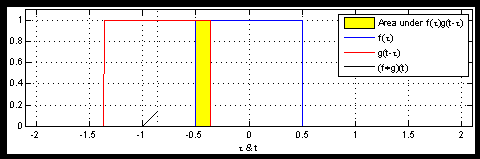
\includegraphics[scale=0.5]{diagrams/conv1}
	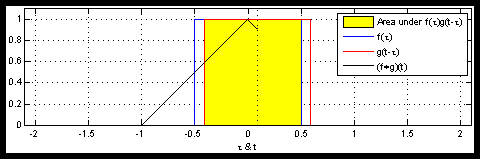
\includegraphics[scale=0.5]{diagrams/conv2}
	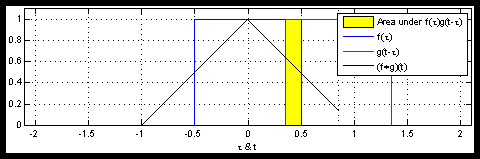
\includegraphics[scale=0.5]{diagrams/conv3}
\end{figure}

Formally this, equates to the following definition for convolution over continuous domains:
\begin{definition}
	The \textbf{convolution} $*$, of two functions $F$ and $G$ is defined as:
	\begin{equation}
		(F*G)(t) = \int_{-\infty}^\infty F(\tau) \;G(t - \tau) \; d\tau
	\end{equation}
\end{definition}
and in the case of discrete linear convolution, summation would replace integration.
In this equation, $t$ represents the translation of $G$ as well as the input for $(F*G)$
while $\tau$ is internal to the integral and varies over the real line.


\begin{figure}[ht]
	\caption[Gaussian Blurring]{512x512px ``Lena''(a) with a 1px (b) and 5px (c) Gaussian blur applied. 
	Gaussian blurring is accomplished by convolving an image with a Gaussian kernel and is commonly used
	in image processing to reduce noise prior to edge detection.
	\label{fig:lennablur}}
	\centering
	\begin{subfigure}[b]{0.3\textwidth}
                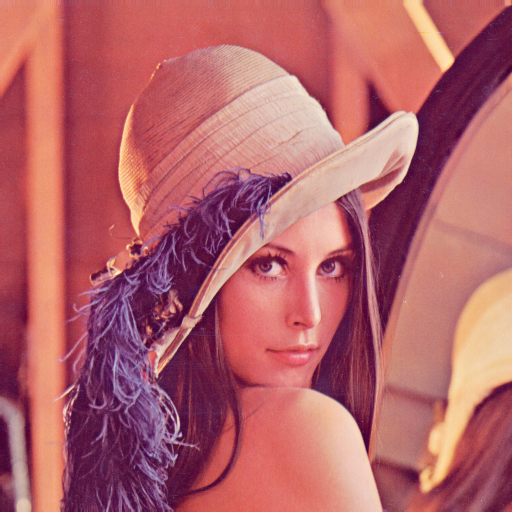
\includegraphics[scale=0.25]{diagrams/Lenna}
                \caption{Original Image}
       \end{subfigure}
       \begin{subfigure}[b]{0.3\textwidth}
                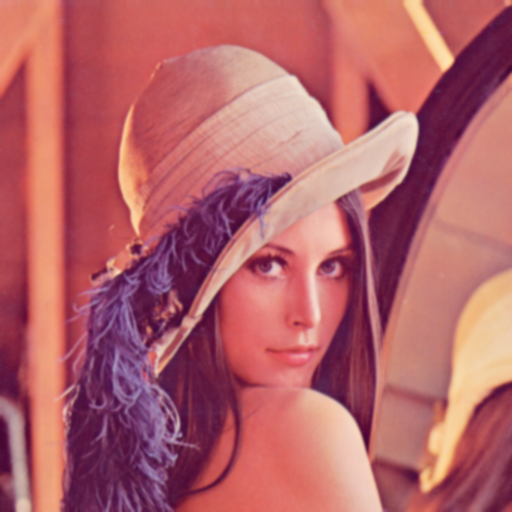
\includegraphics[scale=0.25]{diagrams/Lenna-blur1}
                \caption{1px Gaussian blur}
       \end{subfigure}
       \begin{subfigure}[b]{0.3\textwidth}
                
\includegraphics[scale=0.25]{diagrams/Lenna-blur5}
                \caption{5px Gaussian blur}
       \end{subfigure}
\end{figure}


Convolution has applications in many areas of mathematics and engineering.
One very common use in image processing is in blurring.
\emph{Gaussian blurring} is the result of a 2-dimensional convolution of an image with the Gaussian distribution function:
\begin{equation}
	G(x,y) = \frac{1}{2 \pi \sigma^2} \; \text{exp} \left( - \frac{x^2 + y^2}{2\sigma^2} \right)
\end{equation}
Blurring an image in this way reduces noise and greatly increases the efficacy of subsequent edge detection.
In statistics, a (simple) \emph{moving average} can be represented as a convolution by a rectangular pulse while more
generally, weighted moving averages can be made by convolving with other functions.





%%%%%%%%%%%%%%%%%%%%%%%%%%%%%%%%%%%%%%%%%
%
% CONVOLUTION OF PIECEWISE
%
%%%%%%%%%%%%%%%%%%%%%%%%%%%%%%%%%%%%%%%%%
\section{Convolution of Piecewise Functions}

CAS such as Maple and Mathematica are quite adept at solving integrals.
Convolution of elementary functions generally poses no problem.
When convolving two piecewise continuous functions, many possible intervals arise and the conditionals that arise
can quickly overwhelm them unaided. \todo{cite, rewrite?}

We are interested in \emph{Symbolic Linear Convolution} (of piecewise continuous functions).
First we consider the typical approach for convolution of ``one piece'' functions 
\cite{evans1994algorithms, west1993symbolic}.
Given two functions, $F$ and $G$ defined as:


\begin{equation}
	F(x)=f^{[a_f,b_f)}(x) = 
		\begin{cases}
			f(x) & a_f \leq x < b_f \\
			0 & \text{otherwise}
		\end{cases}
\end{equation}

\begin{equation}
	G(x)=g^{[a_g,b_g)}(x) = 
		\begin{cases}
			g(x) & a_g \leq x < b_g \\
			0 & \text{otherwise}
		\end{cases}
\end{equation}
we would like to compute the convolution $(F*G)$.
In addition, we generally assume that $b_f - a_f \leq b_g - a_g$ (i.e. $F$ is non-zero over a shorter interval).
If this is not the case, convolution is commutative so we simply rearrange: $F * G = G * F$.
To see this, simply apply the substitute $\tau' = t-\tau$ in equation (7.1):
\begin{equation}
	(F*G)(t) = \int_{-\infty}^\infty F(\tau) G(t-\tau) \;d \tau = \int_{\infty}^{-\infty} F(t-\tau')G(\tau')\; (-1) d\tau' = (G*F)(t)
\end{equation}

Thus we can assume that our static function is also the function with the shorter interval.
Since $F$ and $G$ are zero outside of their respective intervals, we do not need to integrate over the entire real line. 
$F$ is our static function, so $[a_f, b_f)$ would be sufficient.
This is still more than we necessarily need though, 

\begin{align}
	(F*G)(t) 
	&= \int_{-\infty}^\infty F(\tau)\; G(t-\tau) \; d\tau \notag \\
	&= \int_{a_f}^{b_f} f(\tau) \; G(t-\tau) \; d\tau \notag \\
	&= 	\begin{cases}
			\int_{a_f}^{x-a_g} f(\tau) \; g(t-\tau) \; d\tau 	& (a_f+a_g) \leq t < (b_f+a_g) \\
			\int_{a_f}^{b_f} f(\tau) \; g(t-\tau) \; d\tau		& (b_f+a_g) \leq t < (a_f+b_g) \\
			\int_{x-b_g}^{b_f} f(\tau) \; g(t-\tau) \; d\tau	& (a_f+b_g) \leq t < (b_f+b_g) \\
			0										& \text{otherwise}
		\end{cases}
\end{align}


This is the way it's typically done.


%%%%%%%%%%%%%%%%%%%%%%%%%%%%%%%%%%%%%%%%%
%
% HYBRID CONVOLUTION
%
%%%%%%%%%%%%%%%%%%%%%%%%%%%%%%%%%%%%%%%%%
\section{Hybrid Function Convolution}

With hybrid functions we do not have to worry about the relative length of $f$ and $g$ intervals.

Instead for hybrid functions $F = f^{[a_f, b_f)}$ and $G = g^{[a_f, b_f)}$:

\begin{align}
	(F \;*\; G) (t) = 
		\mathcal{R}_+ &\left( \; \left( 
			\int_{a_f}^{x-a_g} f(\tau) \; g(t-\tau) \; d\tau \right)^{[\![a_f+a_g,\; b_f+a_g)\!)} 
				\right. \notag \\ &\oplus \left( 
			\int_{a_f}^{b_f} f(\tau) \; g(t-\tau) \; d\tau \right)^{[\![b_f+a_g,\; a_f+b_g)\!)} 
				\notag \\ &\oplus \left. \left( 
			\int_{x-b_g}^{b_f} f(\tau) \; g(t-\tau) \; d\tau \right)^{[\![a_f+b_g,\; b_f+b_g)\!)} 
				\; \right)(t)
\end{align}

When $b_f - a_f \leq b_g - a_g$ then the intervals will be disjoint and the expression is identical to 2.61

Otherwise, the interval $[\![b_f +a_g, \; a_f + b_g)\!)$ will have a negative orientation.

For $(a_f+b_g) \leq t < (b_f+a_g)$ then $t$ will be in all three regions and we have


%%%%%%%%%%%%%%%%%%%%%%%%%%%%%%%%%%%%%%%%%
%
% INFINITE INTERVALS
%
%%%%%%%%%%%%%%%%%%%%%%%%%%%%%%%%%%%%%%%%%
\section{Infinite Intervals}



%%%%%%%%%%%%%%%%%%%%%%%%%%%%%%%%%%%%%%%%%
%
% EXAMPLE
%
%%%%%%%%%%%%%%%%%%%%%%%%%%%%%%%%%%%%%%%%%
\section{Example}

\newpage